% Op icon: bezier — curve with its dashed control polygon and control points.
\documentclass[tikz,border=2mm]{standalone}
\usetikzlibrary{arrows.meta,calc,shapes.geometric}
\begin{document}
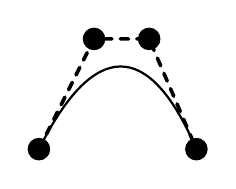
\begin{tikzpicture}[line width=1.3pt, line cap=round, line join=round, >=Stealth, x=1mm,y=1mm]
  \draw[dashed] (-10,-6) -- (-3,8) -- (4,8) -- (10,-6);
  \draw[thick] (-10,-6) .. controls (-3,8) and (4,8) .. (10,-6);
  \foreach \p in {(-10,-6),(-3,8),(4,8),(10,-6)} { \filldraw \p circle (1.2); }
\end{tikzpicture}
\end{document}
